\chapter{Despacho económico a corto plazo.}
	\section{Despacho económico diario de generación. Mercado diario.}
		\textbf{Objetivo:} repartir la demanda total del sistema $P_D\,[MW]$ entre los generadores disponibles, de forma que el coste total de generación, en $\dfrac{\euro}{MWh\cdot \text{día}}$, sea el mínimo posible, con las mínimas pérdidas en la red y menores emisiones de $CO_{2,eq}$.
		
		
		El \textbf{coste total de generación} es variable en cada hora, debido a que las centrales que intervienen tienen eficiencias y costes muy distintos.
		
		
		La resolución del despacho económico (D.E.) considera una serie de \textbf{restricciones técnicas} que limitan el uso de las centrales.
		
		
		Es necesario considerar la opción de \textbf{acoplar o desacoplar los grupos de generación} según la variación de la demanda.
		
		
		\textbf{Programación Horaria de Grupos Térmicos:} problema de operar un sistema de energía eléctrica a coste mínimo, debido a que
		
		\begin{itemize}
			\item[-] los costes fijos de operación de una central térmica pueden ser comparativamente altos, luego no es viable operar a un nivel de producción bajo \textrightarrow Desacoplar centrales cuando hay baja demanda.
			\item[-] las energías renovables ofertan a coste 0.
			\item[-] las centrales nucleares ofertan a coste casi 0 (por considerarse no regulables).
		\end{itemize}
		
		
		\textbf{Coordinación hidráulica:} contribuye a la disminución de los costes de generación en horas punta.
	
		\subsection{Problema de optimización.}
			Sea un sistema eléctrico con $m$ generadores y $n$ nudos. La resolución de un \textbf{flujo de carga óptimo} (OPF, Optimal Power Flow) consiste en elegir las potencias $P_{G_i}$ de los $m$ generadores disponibles y los módulos de las tensiones $U_i$ en los $n$ nudos, de forma que se minimice el coste total de generación $C_T$:
			
			\[C_T = \sum_{i = 1}^m C_i\,\left[\dfrac{\euro}{h}\right] \Rightarrow 
			OPF = \min{ \left\{ \sum_{i = 1}^n C_{G_i} (P_{G_i}) \right\} } \]
			
			
			Son problemas de \textbf{optimización lineal}, \textbf{lineal entera mixta} o \textbf{no lineal} cuando se tienen en cuenta las pérdidas eléctricas, sujetos a restricciones. 
			
		\subsection{Restricciones en la optimización.}
			Las potencias generadas por cada grupo deben estar comprendidas entre un \textbf{límite mínimo}, dado por la \textbf{turbina}, y un \textbf{máximo}, dado por el \textbf{generador}.
			
			
			El flujo de potencia activa y reactiva en cada línea no puede superar un valor máximo por motivos de la capacidad de la línea.
			
			
			La tensión en los nudos del sistema no debe quedar fuera de los límites impuestos por la calidad de suministro (en redes de transporte de 220-400 kV).
			
			
			\begin{table}[H]
				\centering
				\begin{tabular}{cc}
					\textbf{Rango de tensión} & \textbf{Periodo de tiempo de funcionamiento}\\
					\hline
					$0.85-0.9\,p.u.$ & 60 minutos\\
					$0.9-1.0875\,p.u.$ & Ilimitado\\
					$1.0875-1.1\,p.u.$ & 60 minutos
				\end{tabular}
				%\caption{Tiempos máximos de caídas de tensión en redes de transporte.}
				\label{tab:tiemposCdt}
			\end{table}
			
			
			La frecuencia en los nudos no debe superar:
			
			\begin{table}[H]
				\centering
				\begin{tabular}{cc}
					\textbf{Rango de frecuencias} & \textbf{Periodo de tiempo de funcionamiento}\\
					\hline
					$47.5-48.5\,Hz$ & 30 minutos\\
					$48.5-49.0\,Hz$ & Ilimitado\\
					$49.0-51.0\,Hz$ & Ilimitado\\
					$51.0-51.5\,Hz$ & 30 minutos
				\end{tabular}
				%\caption{Tiempos máximos de caídas de tensión en redes de transporte.}
				\label{tab:tiemposfrecuencias}
			\end{table}			
			
		\subsection{Curva de consumo de las unidades térmicas generadoras.}
			Una central térmica generadora queda descrita por:
			\begin{itemize}
				\item Cantidad de calor de entrada requerido: $H_{G_i}\,\left[\dfrac{MJ}{h}\right]$.
				\item Cantidad de energía eléctrica entregada (trifásica): $P_{G_i}\,[MW]$.
			\end{itemize}
			
			\[H_{G_i} = \alpha_i + \beta_i \cdot P_{G_i} + \gamma_i \cdot P_{G_i}^2\,\left[\dfrac{MJ}{h}\right]\]
			
			\begin{itemize}
				\item $\alpha_i$ son los costes fijos $[\euro/h]$ de operación (salarios de los trabajadores) y consumo de combustible de autoconsumo cuando la producción es 0.
				\item $\beta_i$ y $\gamma_i$ son parámetros positivos que caracterizan la dependencia de la curva de costes o de consumo con su nivel de generación.
			\end{itemize}
			
			\begin{figure}[H]
				\begin{minipage}{0.4\textwidth}
					\begin{figure}[H]
						\centering
							\begin{circuitikz}[scale = 0.5]
								\tikzstyle{every node}=[font=\normalsize]
								\draw [->, >=Stealth] (3.5,10.25) -- (3.5,16)node[pos=1,right]{$H_{G_i}\,[MW/h]$};
								\draw [->, >=Stealth] (3.5,10.25) -- (9.5,10.25)node[pos=1,right]{$P_{G_i}\,[MW]$};
								\draw [ color={rgb,255:red,0; green,128; blue,255}, short] (3.5,11.25) .. controls (6.5,11.5) and (8,11.75) .. (9,15.25);
								\draw [dashed] (4.5,11.25) -- (4.5,10.25)node[pos=1,below]{$P_{G_i}^{min}$};
								\draw [dashed] (8.5,13.75) -- (8.5,10.25)node[pos=1,below]{$P_{G_i}^{max}$};
							\end{circuitikz}
						
						\label{fig:my_label}
					\end{figure}
				\end{minipage}
				\begin{minipage}{0.6\textwidth}
					Esta es la función que define la \textbf{curva de consumo}, y expresa la cantidad de combustible consumido por hora en función de la producción eléctrica. Mide la eficiencia de la unidad de producción. Puede ser continua o a tramos.
				\end{minipage}
			\end{figure}
			
			Esta curva se obtiene de pruebas que se le realizan al grupo turbina-generador para varios niveles de salida: 100, 75, 50 y 25\%, por ejemplo.
	
	\section{Despacho de generación: despacho económico (D.E.).}
		\subsection{Característica de coste de las unidades térmicas generadoras.}
			Multiplicando la cantidad de calor $H_{G_i}$ por el coste de combustible se obtiene la función de coste total de cada unidad de producción $C_i(P_{G_i})$, en $\euro/h$ y en función de $P_{G_i}$.
			
			\begin{figure}[H]
				\begin{minipage}{0.4\textwidth}
					\begin{figure}[H]
						\centering
						\begin{circuitikz}[scale = 0.5]
							\tikzstyle{every node}=[font=\normalsize]
							\draw [->, >=Stealth] (3.5,10.25) -- (3.5,16)node[pos=1,right]{$C_i(P_{G_i})\,[\euro/h]$};
							\draw [->, >=Stealth] (3.5,10.25) -- (9.5,10.25)node[pos=1,right]{$P_{G_i}\,[MW]$};
							\draw [ color={rgb,255:red,0; green,128; blue,255}, short] (3.5,11.25) .. controls (6.5,11.5) and (8,11.75) .. (9,15.25);
							\draw [dashed] (4.5,11.25) -- (4.5,10.25)node[pos=1,below]{$P_{G_i}^{min}$};
							\draw [dashed] (8.5,13.75) -- (8.5,10.25)node[pos=1,below]{$P_{G_i}^{max}$};
						\end{circuitikz}
						
						\label{fig:my_label}
					\end{figure}
				\end{minipage}
				\begin{minipage}{0.6\textwidth}
					El coste total incluye un coste fijo (que no contiene coste de inversión), costes de operación fijos, consumos propios y costes variables de O\&M, combustible, emisiones de $CO_2$, etc. Los costes variables son dependientes de la potencia activa trifásica que entrega el generador. Las centrales hidráulicas tienen una curva similar en función del caudal turbinado.
				\end{minipage}
			\end{figure}
			
			Si la curva de consumo es una función cuadrática admite soluciones analíticas:
			\[C_i(P_{G_i}) = \alpha_i + \beta_i\cdot P_{G_i} + \gamma_i\cdot P_{G_i}^2\]
			
		\subsection{Conversión de la curva de consumo específico a curva de costes.}
			$1\,th = 1.162\,kWh = 1000\,kcal$
			
			$1\,kWh = 0.86\,th$
			
			$1\,tep = 11.627\,MWh = 10^4\,th$
			
			$1\,kJ = 9.5\,th$
			
		\subsection*{Ejemplo.}
			Una central térmica de carbón, con un PCI de $6050\,th/t$ tiene un coste de $37.91\,\euro/t$. Obtener la curva de coste del generador.
			\[C_1\,\left[\dfrac{\euro}{h}\right] = \dfrac{H_1\,\left[\dfrac{th}{h}\right]}{6050\,\left[\dfrac{th}{t}\right]} \cdot 37.91\,\left[\dfrac{\euro}{t}\right] = 426.56 + 10.756\cdot P_{G_1} + 0.0031\cdot P_{G_1}^2\]
			
		\subsection{Restricciones técnicas de la curva de coste o consumo.}
			\begin{itemize}
				\item Límites operativos:
				\begin{itemize}
					\item Potencia mínima (por caldera y turbina).
					\item Potencia máxima (por generador síncrono).
				\end{itemize}
				
				\item Tiempo mínimo de operación.
				\item Tiempo mínimo de arranque.
				\item Tiempo de respuesta entre intervalos horarios: Rampa de subida y bajada [MW/h].
				\item Coste de arranque.
				\item Coste de parada.
				\item Penalizaciones por emisiones de $CO_2$.
			\end{itemize}
			
		\subsection{Consumo específico o \textit{Heat Rate} (H.I.).}
			Es la medida del rendimiento de una central termoeléctrica. Se define por el cociente entre la energía térmica aportada en forma de combustible y la energía generada en bornes del generador.
			
			\[HR = \dfrac{H_{G_i}}{P_{G_i}} = \dfrac{\alpha_i}{P_{G_i}} + \beta_i + \gamma_i\cdot P_{G_i}\]
			
			\begin{figure}[H]
				\centering
					\begin{circuitikz}
						\tikzstyle{every node}=[font=\normalsize]
						\draw [->, >=Stealth] (3.5,10.25) -- (3.5,16)node[pos=1,above]{$HR\,\left[\dfrac{MJ}{MWh}\right]$};
						\draw [->, >=Stealth] (3.5,10.25) -- (9.5,10.25)node[pos=1,right]{$P_{G_i}\,[MW]$};
						\draw [ color={rgb,255:red,0; green,128; blue,255}, short] (4.5,15.25) .. controls (6,11.5) and (8,11.75) .. (8.5,13.25);
						\draw [dashed] (4.5,15.25) -- (4.5,10.25)node[pos=1,below]{$P_{G_i}^{min}$};
						\draw [dashed] (8.5,13.25) -- (8.5,10.25)node[pos=1,below]{$P_{G_i}^{max}$};
						\draw [dashed] (7.25,12.25) -- (7.25,10.25)node[pos=1,below]{$P_{ef}$};
						\draw [dashed] (7.25,12.25) -- (3.5,12.25);
						\draw (7.25,12.25) to[short, -*] (7.25,12.25);
					\end{circuitikz}
				
				\label{fig:my_label}
			\end{figure}
			
			La máxima eficiencia de la unidad se obtiene en el mínimo de la función HR, que se da para valores próximos a la potencia máxima del generador.
			
			\begin{figure}
				\begin{minipage}{0.5\textwidth}
					\[\eta = \dfrac{3600}{HR}\,\left[\dfrac{MWh_e}{MWh_t}\right]\]
				\end{minipage}
				\begin{minipage}{0.5\textwidth}
					\[HR = \dfrac{3600}{\eta}\,\left[\dfrac{MJ}{MWh}\right]\]
				\end{minipage}
			\end{figure}
			
			\begin{figure}[H]
				\centering
					\begin{circuitikz}[scale = 0.7]
						\tikzstyle{every node}=[font=\normalsize]
						\draw [->, >=Stealth] (3.5,10.25) -- (3.5,16)node[pos=1,right]{$\eta\,[\%]$};
						\draw [->, >=Stealth] (3.5,10.25) -- (9.5,10.25)node[pos=1,right]{$P_{G_i}\,[MW]$};
						\draw [ color={rgb,255:red,0; green,128; blue,255}, short] (4.25,11.25) .. controls (4.75,13.75) and (6.5,15) .. (8.75,15);
						\draw [->, >=Stealth] (12.5,10.25) -- (12.5,16.25)node[pos=1,right]{$HR\,\left[\dfrac{MJ}{MWh}\right]$};
						\draw [->, >=Stealth] (12.5,10.25) -- (18.25,10.25)node[pos=1,right]{$P_{G_i}\,[MW]$};
						\draw [ color={rgb,255:red,0; green,128; blue,255}, short] (13.5,15) .. controls (14,12.5) and (15.25,11.5) .. (17.5,11.25);
					\end{circuitikz}
				
				\label{fig:my_label}
			\end{figure}
			
		\subsection*{Ejemplo.}
			Cálculo del HR para una turbina de gas.
		
		
			\textbf{Ojo:} el HR de la turbina determinado mediante pruebas es distinto del $H\!R_{ISO}$ que proporciona el fabricante.
			
			
			\textbf{Datos:} 
			
			
			\renewcommand{\arraystretch}{1.2}
			\centering
			\begin{tabular}{llc}
				\textbf{Característica TG} & \textbf{Unidades} & \textbf{Valor}\\
				\hline
				Temperatura ambiente & $^\circ C$ & 15\\
				\hline
				Presión atmosférica & $mbar$ & 1013\\
				\hline
				\multirow{2}{*}{$HR_{ISO}$} & \multirow{2}{*}{$\dfrac{kJ}{kWh}$} & \multirow{2}{*}{9526}\\
				&&\\
				\hline
				\multirow{2}{*}{PCI} & \multirow{2}{*}{$\dfrac{MJ}{Nm^3}$} & \multirow{2}{*}{35.5}\\
				&&\\
				\hline
				Potencia eléctrica neta (ISO) & $MW$ & 240
			\end{tabular}
			
			\begin{figure}[H]
				\centering
				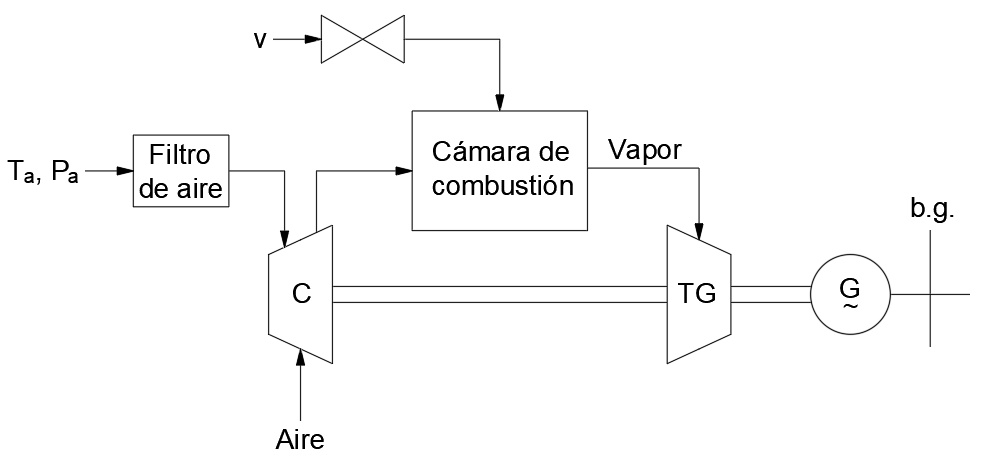
\includegraphics[width=0.7\linewidth]{res/tema5/turbinaGas}
				\label{fig:turbinagas}
			\end{figure}
			
	
	\section{Coste total de producción del sistema eléctrico.}
		\subsection{}
	
	\section{Coste incremental de la generación.}
		\subsection{}
	
	\section{Despacho económico con pérdidas en la red.}
		\subsection{}
	
	\section{Programación de arranques y paradas de centrales.}
		\subsection{}
	